\tikzset{
	main/.style={black, line width=0.4mm, opacity=1},
	second/.style={gray, opacity=5},
	arrow/.style={-latex, shorten >=1ex, shorten <=1ex, bend angle=45}
}
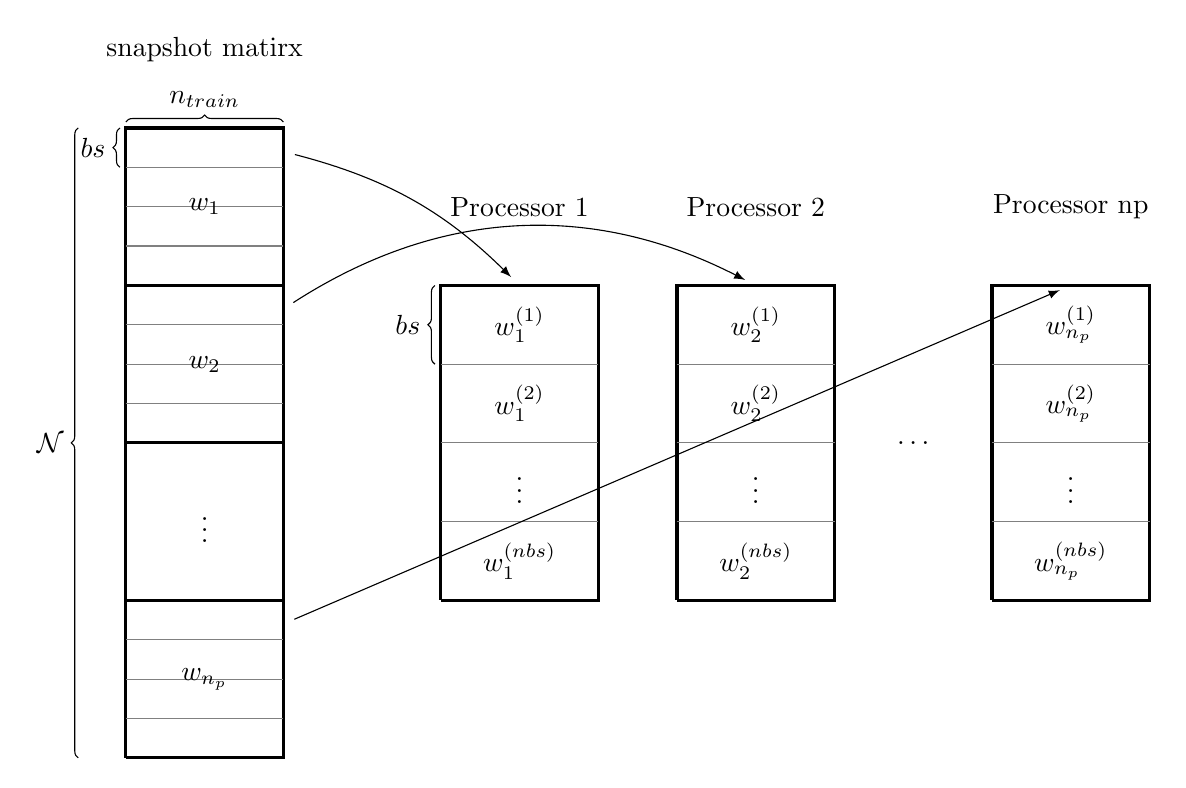
\begin{tikzpicture}
%% Snapshot Matrix
\draw (1,9) node {snapshot matirx};
\draw[main] (0,0) -- (2,0) -- (2,8)-- (0,8)-- (0,0);
\draw[main] (0,2) -- (2,2) ;
\draw[main] (0,4) -- (2,4) ;
\draw[main] (0,6) -- (2,6) ;

\draw[second] (0,7.5) -- (2,7.5) ;
\draw[second] (0,7) -- (2,7) ;
\draw[second] (0,6.5) -- (2,6.5) ;

\draw[second] (0,5.5) -- (2,5.5) ;
\draw[second] (0,5) -- (2,5) ;
\draw[second] (0,4.5) -- (2,4.5) ;

\draw[second] (0,1.5) -- (2,1.5) ;
\draw[second] (0,1) -- (2,1) ;
\draw[second] (0,.5) -- (2,.5) ;

\draw[decorate, decoration={brace,mirror}, yshift=.5ex]  (2,8) -- node[above=0.4ex] {$n_{train}$}  (0,8);
\draw[decorate, decoration={brace}, xshift=-4ex]  (0,0) -- node[left=0.4ex] {$\mathcal{ N }$}  (0,8);
\draw[decorate, decoration={brace}, xshift=-.5ex]  (0,7.5) -- node[left=0.4ex] {$bs$}  (0,8);

\draw (1,7) node {$w_1$};
\draw (1,5) node {$w_2$};
\draw (1,3) node {$\vdots$};
\draw (1,1) node {$w_{n_p}$};

%% prozessor1 Matrix
\draw (5,7) node {Processor 1};
\draw[main] (4,2) -- (6,2) -- (6,6)-- (4,6)-- (4,2);
\draw[second] (4,3) -- (6,3) ;
\draw[second] (4,4) -- (6,4) ;
\draw[second] (4,5) -- (6,5) ;

\draw (5,5.5) node {$w_1^{(1)}$};
\draw (5,4.5) node {$w_1^{(2)}$};
\draw (5,3.5) node {$\vdots$};
\draw (5,2.5) node {$w_{1}^{(nbs)}$};

\draw[decorate, decoration={brace}, xshift=-.5ex]  (4,5) -- node[left=0.4ex] {$bs$}  (4,6);

%% prozessor2 Matrix
\draw (8,7) node {Processor 2};
\draw[main] (7,2) -- (9,2) -- (9,6)-- (7,6)-- (7,2);
\draw[second] (7,3) -- (9,3) ;
\draw[second] (7,4) -- (9,4) ;
\draw[second] (7,5) -- (9,5) ;

\draw (8,5.5) node {$w_2^{(1)}$};
\draw (8,4.5) node {$w_2^{(2)}$};
\draw (8,3.5) node {$\vdots$};
\draw (8,2.5) node {$w_{2}^{(nbs)}$};

%% Dots
\draw (10,4) node {$\dots$};

%% prozessor np Matrix
\draw (12,7) node {Processor np};
\draw[main] (11,2) -- (13,2) -- (13,6)-- (11,6)-- (11,2);
\draw[gray] (11,3) -- (13,3) ;
\draw[gray] (11,4) -- (13,4) ;
\draw[gray] (11,5) -- (13,5) ;

\draw (12,5.5) node {$w_{n_p}^{(1)}$};
\draw (12,4.5) node {$w_{n_p}^{(2)}$};
\draw (12,3.5) node {$\vdots$};
\draw (12,2.5) node {$w_{n_p}^{(nbs)}$};

%% Pfeile
\draw [arrow, bend angle=15, bend left]  (2,7.7) to (5,6);
\draw [arrow, bend angle=30, bend left]  (2,5.7) to (8,6);

\draw [arrow, ]  (2,1.7) to (12,6);


\end{tikzpicture}